\documentclass[tikz,border=3pt]{standalone}
\usepackage{tikz-feynman}
\begin{document}
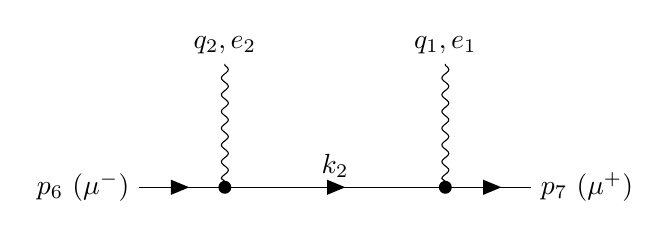
\begin{tikzpicture}
\begin{feynman}
\vertex (p6) {\(p_6\) (\(\mu^-\))};
\vertex[right=1.8cm of p6, dot] (A) {};
\vertex[right=2.8cm of A, dot] (B) {};
\vertex[right=1.8cm of B] (p7) {\(p_7\) (\(\mu^+\))};
\vertex[above=1.8cm of A] (q2) {\(q_2,e_2\)};
\vertex[above=1.8cm of B] (q1) {\(q_1,e_1\)};

\diagram* {
  (p6) -- [fermion] (A) -- [fermion, edge label=\(k_2\)] (B) -- [fermion] (p7),
  (q2) -- [photon] (A),
  (q1) -- [photon] (B),
};
\end{feynman}
\end{tikzpicture}
\end{document}
